\clearpage
\makeatletter
\efloat@restorefloats
\makeatother


\begin{appendix}
\section{}
\hypertarget{experiments-included-in-the-linear-mixed-effects-model.}{%
\subsection{Experiments included in the linear mixed-effects
model.}\label{experiments-included-in-the-linear-mixed-effects-model.}}

The selected experiments consist of an artificial grammar learning task
with 12-month-old infants. These experiments are characterized by
variability in the number of infants' prior HPP visits\footnote{At the
  time of publication of Saffran \& Wilson (2003), the first author
  noted that there appeared to be an association between the number of
  prior studies completed by the infants and the direction of
  preference. The analysis was included in the original manuscript
  submission but was removed from later revisions based on the
  manuscript reviews.}. They include all studies run in the two senior
authors' labs that included (a) 12- to 13-month-old participants; (b)
HPP; (c) artificial grammar learning (linguistic or non-linguistic); (d)
2 to 5 minutes of exposure; (e) an \emph{a priori} hypothesis that
infants would show learning; (f) visit numbers recorded at the time of
testing. The studies are thus as well matched as is possible given the
retrospective nature of this analysis.

\emph{Saffran \& Wilson (2003)} demonstrated that 12-month-old infants
can compute multiple regularities from a finite-state grammar. Infants
were able to first segment words from running speech based on
transitional probabilities, then detect permissible orderings of the
segmented words. Test items consisted of grammatical and ungrammatical
sentences that could only be discriminated based on word-level
information (transitional probabilities between syllables were not
informative about the ``grammaticality'' of test items). Infants showed
a significant familiarity preference: \emph{F}(1, 38)= 5.37,
\emph{p}\textless{}.05.

\emph{Saffran et al. (2008)} demonstrated that infants could detect
simple phrases (i.e., clusters of nonsense words grouped together based
on statistical regularities) from artificial grammars. In Exp. 1,
infants in the Predictive Language condition were familiarized with a
grammar including predictive (statistical) dependencies between words.
The test items consisted of familiar sentences vs.~novel sentences
violating the grammar. Infants showed a significant novelty preference:
\emph{t}(11)= 2.52, \emph{p}\textless{}.05.

\emph{Santolin \& Saffran (2019)} is a conceptual replication of Saffran
et al. (2008) using non-linguistic sounds (e.g., computer alert sounds)
to implement the grammars. Infants exposed to the Predictive language
showed a significant novelty preference: \emph{t}(26)=2.45,
\emph{p}=.021, \emph{d}=0.47.

We replicated the Predictive Language condition of Santolin \& Saffran
(2019) at the University Pompeu Fabra, Barcelona (Santolin et al.,
2019), using identical stimuli and procedures. We found significant
discrimination of the test stimuli but observed the opposite direction
of preference: Infants listened longer to familiar than novel strings:
\emph{t}(23)=2.30, \emph{p}=.030, \emph{d}=0.47. All results are shown
in Fig. 1 of the main manuscript.

\hypertarget{participants-information}{%
\subsection{Participants information}\label{participants-information}}

We retrieved data from 102 12-month-old infants who had participated in
a range of 1-6 studies. Three of the studies were run in Madison, WI
(University of Wisconsin-Madison): Saffran \& Wilson, 2003 (Exp. 2):
\emph{N}=40, mean age: 11.5 months; Saffran et al., 2008 (Exp. 1,
Condition P-Language): \emph{N}=12), mean age: 12.8 months; Santolin \&
Saffran, 2019 (Condition 1); \emph{N}=26, mean age: 12.9 months. One
study was run in Barcelona, Spain (Universitat Pompeu Fabra): Santolin,
Saffran \& Sebastian-Galles, 2019: \emph{N}=24, mean age: 13 months. Two
data points (average looking time for familiar and novel test items)
were available for each participant. Participants included in the
current analysis are those included in the final version of the studies.

\hypertarget{linear-mixed-effects-model---additional-information}{%
\subsection{Linear mixed-effects model - additional
information}\label{linear-mixed-effects-model---additional-information}}

We fit a model predicting looking time (\(LT\)) including \(TestItem\)
(Familiar vs.~Novel), number of Head-turn Preference Procedure
experiments completed by infants (\(HPP\)), and their interaction
(\(Item \times HPP\)) as fixed effects. Participant and study (4 levels:
Santolin \& Saffran (2019), Santolin et al. (2019), Saffran et al.
(2008), and Saffran \& Wilson (2003)) were included as random effects.
Following Barr, Levy, Scheepers, \& Tily (2013), we fit a model with a
maximal random effects structure including random intercepts
by-participant and by-study, and random slopes of HPP by-participant and
by-study. However, due to lack of convergence, we pruned the random
effects structure until convergence was achieved (e.g., Brauer \&
Curtin, 2018). The final model included by-participant and by-study
random intercepts only. The particular random effects structure chosen
does not qualitatively impact the estimates and conclusions from the
model. This model accounts for cross-participant variability in overall
looking time (as some infants look longer than others), and for
cross-studies differences in overall looking time. The model was fit
using the \texttt{lme4} package (Bates, Mächler, Bolker, \& Walker,
2015) from the R environment (R Core Team, 2018). We used the
\texttt{Anova} function from the \texttt{car} R package (Fox \&
Weisberg, 2019) to perform F-tests on fixed effects using
Kenward-Roger's approximation to degrees of freedom (e.g., Judd,
Westfall, \& Kenny, 2012).

\hypertarget{results-sub-setting-data-to-participants-with-less-than-6-5-4-and-3-hpp-studies}{%
\subsection{Results sub-setting data to participants with less than 6,
5, 4, and 3 HPP
studies}\label{results-sub-setting-data-to-participants-with-less-than-6-5-4-and-3-hpp-studies}}

Consistent with the results of the entire dataset, we found a
statistically significant interaction of \emph{Test Item} with the
number of \emph{HPP} visits when reducing the sample to the infants who
participanted in less than 6, 5, 4, and 3 HPP experiments. Below, we
report the output of the linear mixed-effects model fitted on the
original and reduced samples (Table @ref(tab:tabA1), Fig.
@ref(fig:figA1)).

\begin{longtable}[]{@{}cccccccc@{}}
\caption{(\#tab:tabA1)Output of the Linear Mixed Effects-Model fitted on
the subsetted data. Results are reported for the original analysis, and
the HPP5, HPP4, HPP3, and HPP2 subsets. Degrees of freedom were
approximated using the Kenward-Roger approach, this sometimes resulting
in non integers.}\tabularnewline
\toprule
\textbf{Subset} & \textbf{Term} & \textbf{Coefficient} &
\textbf{\emph{SEM}} & \textbf{95\% CI} & \textbf{F} & \textbf{Den.
\emph{df}} & \textbf{\emph{p}}\tabularnewline
\midrule
\endfirsthead
\toprule
\textbf{Subset} & \textbf{Term} & \textbf{Coefficient} &
\textbf{\emph{SEM}} & \textbf{95\% CI} & \textbf{F} & \textbf{Den.
\emph{df}} & \textbf{\emph{p}}\tabularnewline
\midrule
\endhead
Original & \emph{Intercept} & 7,679.1 & 673.1 & {[}6390.1, 9294.1{]} &
124.6893997 & 9.064502 & \textless{} .001\tabularnewline
& \emph{Test Item} & -1,398.8 & 411.3 & {[}-2204.8, -589.1{]} &
11.5654404 & 100.000000 & .001\tabularnewline
& \emph{HPP} & -539.7 & 238.7 & {[}-999.9, -74.8{]} & 4.8005476 &
133.099688 & .030\tabularnewline
& \emph{Test Item \(\times\) HPP} & 667.1 & 192.6 & {[}247.2, 1028.5{]}
& 11.9927376 & 100.000000 & .001\tabularnewline
HPP 1-5 & \emph{Intercept} & 7,675.0 & 691.6 & {[}6452.7, 9029.3{]} &
118.3288753 & 10.074791 & \textless{} .001\tabularnewline
& \emph{Test Item} & -1,416.1 & 435.4 & {[}-2237.7, -543.7{]} &
10.5777662 & 99.000000 & .002\tabularnewline
& \emph{HPP} & -535.6 & 261.2 & {[}-1081.1, -37.5{]} & 3.9653404 &
133.567312 & .048\tabularnewline
& \emph{Test Item \(\times\) HPP} & 677.8 & 211.3 & {[}241, 1081.9{]} &
10.2938879 & 99.000000 & .002\tabularnewline
HPP 1-4 & \emph{Intercept} & 7,611.1 & 719.4 & {[}6188.4, 9275.6{]} &
107.3503715 & 10.458693 & \textless{} .001\tabularnewline
& \emph{Test Item} & -1,491.1 & 452.1 & {[}-2348.4, -578.5{]} &
10.8789948 & 98.000000 & .001\tabularnewline
& \emph{HPP} & -500.8 & 278.7 & {[}-1070.2, 98.2{]} & 3.0430523 &
131.918391 & .083\tabularnewline
& \emph{Test Item \(\times\) HPP} & 726.2 & 224.9 & {[}294.2, 1145{]} &
10.4251927 & 98.000000 & .002\tabularnewline
HPP1-3 & \emph{Intercept} & 7,470.0 & 794.6 & {[}6007.1, 9172.5{]} &
83.7790216 & 14.299003 & \textless{} .001\tabularnewline
& \emph{Test Item} & -1,349.9 & 532.3 & {[}-2426.9, -267.6{]} &
6.4305807 & 92.000000 & .013\tabularnewline
& \emph{HPP} & -395.8 & 366.6 & {[}-1182.6, 316.1{]} & 1.0867433 &
122.312388 & .299\tabularnewline
& \emph{Test Item \(\times\) HPP} & 627.9 & 294.1 & {[}3, 1252.6{]} &
4.5589727 & 92.000000 & .035\tabularnewline
HPP 1-2 & \emph{Intercept} & 7,301.9 & 1,009.9 & {[}5252.9, 9362.1{]} &
48.8571582 & 23.938709 & \textless{} .001\tabularnewline
& \emph{Test Item} & -1,783.7 & 726.7 & {[}-3199.6, -360.7{]} &
6.0247027 & 78.000000 & .016\tabularnewline
& \emph{HPP} & -261.3 & 586.8 & {[}-1449.8, 991.7{]} & 0.1855918 &
106.961951 & .667\tabularnewline
& \emph{Test Item \(\times\) HPP} & 969.5 & 481.8 & {[}38.3, 2010.4{]} &
4.0493079 & 78.000000 & .048\tabularnewline
\bottomrule
\end{longtable}

In all models, the \(Item \times HPP\) interaction term was
statistically significant {[}HPP 1-5: \emph{F}(1, 99) = 10.29, \emph{p}
= .002; HPP 1-4: \emph{F}(1, 98) = 10.43, \emph{p} = .002; HPP 1-3:
\emph{F}(1, 92) = 4.56, \emph{p} = .035; HPP 1-2: \emph{F}(1, 78) =
4.05, \emph{p} = .048{]} . These results provide evidence that the
effect of HPP on the preference pattern we observed in our main analysis
is not entirely dependent on any subsample of the HPP variable.

\begin{figure}
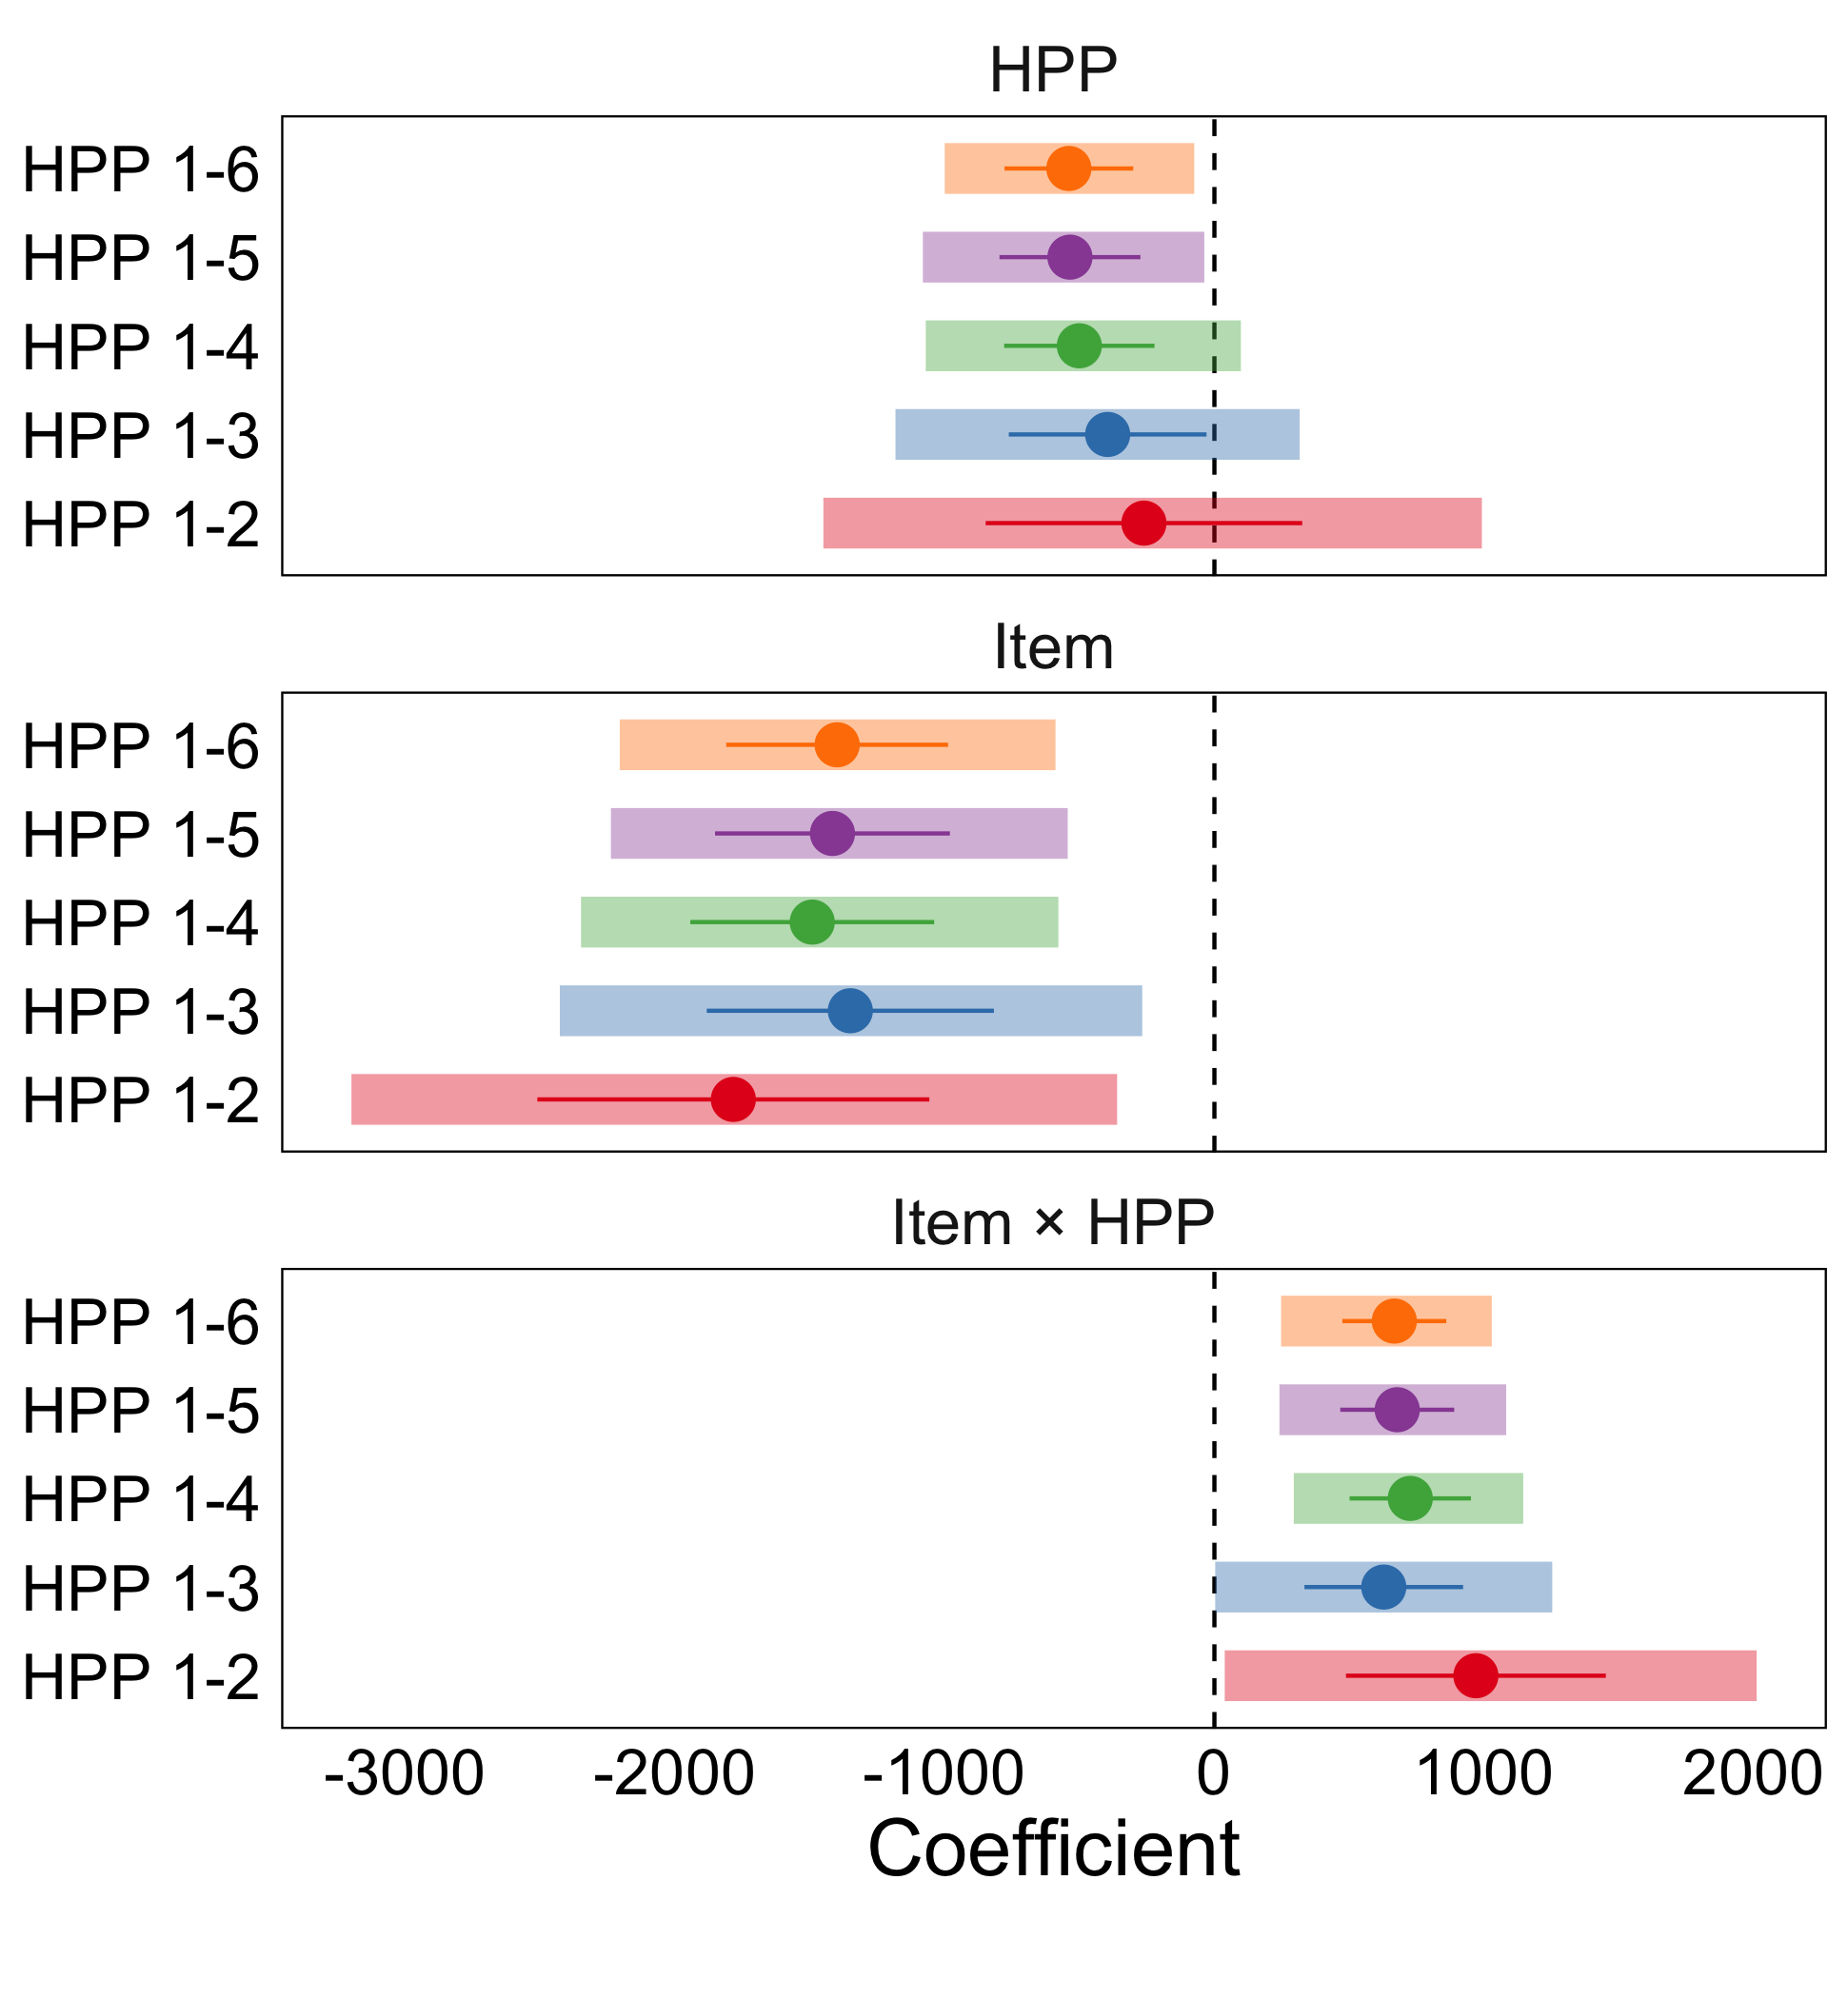
\includegraphics[width=\textwidth]{/Users/GonzaloGGC/projects/Flip/Figures/05_anova-merged} \caption{Graphical representation of the coefficients of the Test Item by HPP visits interaction term of the model fitted on the complete data-set (reported in the main manuscript), and of the models fitted on the reduced data-sets. Black dots represent the point estimate of the coefficient, black whiskers represent the standard error of the mean, and grey boxes represent the bootstrapped 95\% confidence interval around the point estimate.}(\#fig:figA1)
\end{figure}

\newpage

\hypertarget{references}{%
\subsection{References}\label{references}}

\begingroup
\setlength{\parindent}{-0.5in}
\setlength{\leftskip}{0.5in}

\hypertarget{refs}{}
\leavevmode\hypertarget{ref-barr2013}{}%
Barr, D. J., Levy, R., Scheepers, C., \& Tily, H. J. (2013). Random
effects structure for confirmatory hypothesis testing: Keep it maximal.
\emph{Journal of Memory and Language}, \emph{68}(3), 255--278.
\url{https://doi.org/10.1016/j.jml.2012.11.001}

\leavevmode\hypertarget{ref-bates2015}{}%
Bates, D., Mächler, M., Bolker, B., \& Walker, S. (2015). Fitting linear
mixed-effects models using lme4. \emph{Journal of Statistical Software},
\emph{67}(1), 1--48. \url{https://doi.org/10.18637/jss.v067.i01}

\leavevmode\hypertarget{ref-brauer2018}{}%
Brauer, M., \& Curtin, J. J. (2018). Linear mixed-effects models and the
analysis of nonindependent data: A unified framework to analyze
categorical and continuous independent variables that vary
within-subjects and/or within-items. \emph{Psychological Methods},
\emph{23}(3), 389--411. \url{https://doi.org/10.1037/met0000159}

\leavevmode\hypertarget{ref-fox2019}{}%
Fox, J., \& Weisberg, S. (2019). \emph{An R companion to applied
regression} (Third). Thousand Oaks CA: Sage. Retrieved from
\url{https://socialsciences.mcmaster.ca/jfox/Books/Companion/}

\leavevmode\hypertarget{ref-judd2012}{}%
Judd, C. M., Westfall, J., \& Kenny, D. A. (2012). Treating stimuli as a
random factor in social psychology: A new and comprehensive solution to
a pervasive but largely ignored problem. \emph{Journal of Personality
and Social Psychology}, \emph{103}(1), 54--69.
\url{https://doi.org/10.1037/a0028347}

\leavevmode\hypertarget{ref-rcoreteam2018}{}%
R Core Team. (2018). \emph{R: A language and environment for statistical
computing}. Vienna, Austria. Retrieved from
\url{https://www.R-project.org/}

\leavevmode\hypertarget{ref-saffran2008}{}%
Saffran, J., Hauser, M., Seibel, R., Kapfhamer, J., Tsao, F., \&
Cushman, F. (2008). Grammatical pattern learning by human infants and
cotton-top tamarin monkeys. \emph{Cognition}, \emph{107}(2), 479--500.
\url{https://doi.org/10.1016/j.cognition.2007.10.010}

\leavevmode\hypertarget{ref-saffran2003}{}%
Saffran, J. R., \& Wilson, D. P. (2003). From Syllables to Syntax:
Multilevel Statistical Learning by 12-Month-Old Infants. \emph{Infancy},
\emph{4}(2), 273--284. \url{https://doi.org/10.1207/S15327078IN0402_07}

\leavevmode\hypertarget{ref-santolin2019}{}%
Santolin, C., \& Saffran, J. R. (2019). Non-Linguistic Grammar Learning
by 12-Month-Old Infants: Evidence for Constraints on Learning.
\emph{Journal of Cognition and Development}, \emph{20}(3), 433--441.
\url{https://doi.org/10.1080/15248372.2019.1604525}

\leavevmode\hypertarget{ref-santolin2019a}{}%
Santolin, C., Saffran, J. R., \& Sebastian-Galles, N. (2019).
Non-linguistic artificial grammar learning in 12-month-old infants: A
cross-lab replication study. In. Potsdam, Germany.

\endgroup
\end{appendix}
